\subsection{ESMF Machine Model and Programming Model}
\label{sec:progmodel}

The ESMF machine model is a generic interface to the structure and 
configuration of a 
computing platform.  The machine model can return information
such as a list of processors on the same node, the number of processors
per node, whether the architecture supports multiple executables 
running on the same processor, etc.  As the ESMF develops, it will be useful
to extend the machine model to include information on typical system
latencies and bandwidths, cache sizes, and other information that 
might be useful for system-aided load balancing and problem mapping.

The ESMF programming model defines abstractions that expose
features of the computing environment to the user.  It must support the 
efficient utilization of system resources such as   
computing hardware, OS, and standard library or vendor-supplied 
software (e.g., MPI or other message-passing software, Posix threads, OMP),
and must present a reasonably simple interface to the application 
developer.  

ESMF abstracts the compute elements over which data and tasks may be
distributed into decomposition elements, or DEs, which
are essentially threads.  For MPP architectures in which there
is tyically one thread per process, the DE degenerates to a process.
Depending on the hardware system, ESMF threads will be to a limited 
extent compatible with user-defined threads.  The user will have 
the option to enable ESMF threading or not.  In the latter case, the
DE again degenerates to a process.

DEs are organized into topologies, such as a 2-D grid, by the Layout 
class.  A user can define their own Layout, or a Layout can be 
constructed automatically in the process of creating a distributed 
grid.  

The Layout for both homogeneous and heterogeneous programming
strategies can be described compactly and precisely by a layout 
tuple (ltuple) of the form: \\
(D_{1}, D_{2}, ... D_{n}), where D_{n} is a representation of
each dimension in the layout.  \\
Each D_{n} takes the form \\
D_{n} = (<R_{1}>(N_{1},C_{1}), <R_{2}>(N_{2},C_{2}), ... <R_{m}>(N_{m},C_{m})<P> \\
where \\
R_{m} = number of repetitions \\
N_{m} = number of DEs \\
C_{m} = connectivity \\
P = periodic boundary \\

Default values for connectivity are: \\
0 = unrelated processes \\
1 = adjacent processes, e.g. processes on the same node\\
2 = shared memory \\

\begin{figure}
\label{fig:layouts}
\scalebox{0.7}{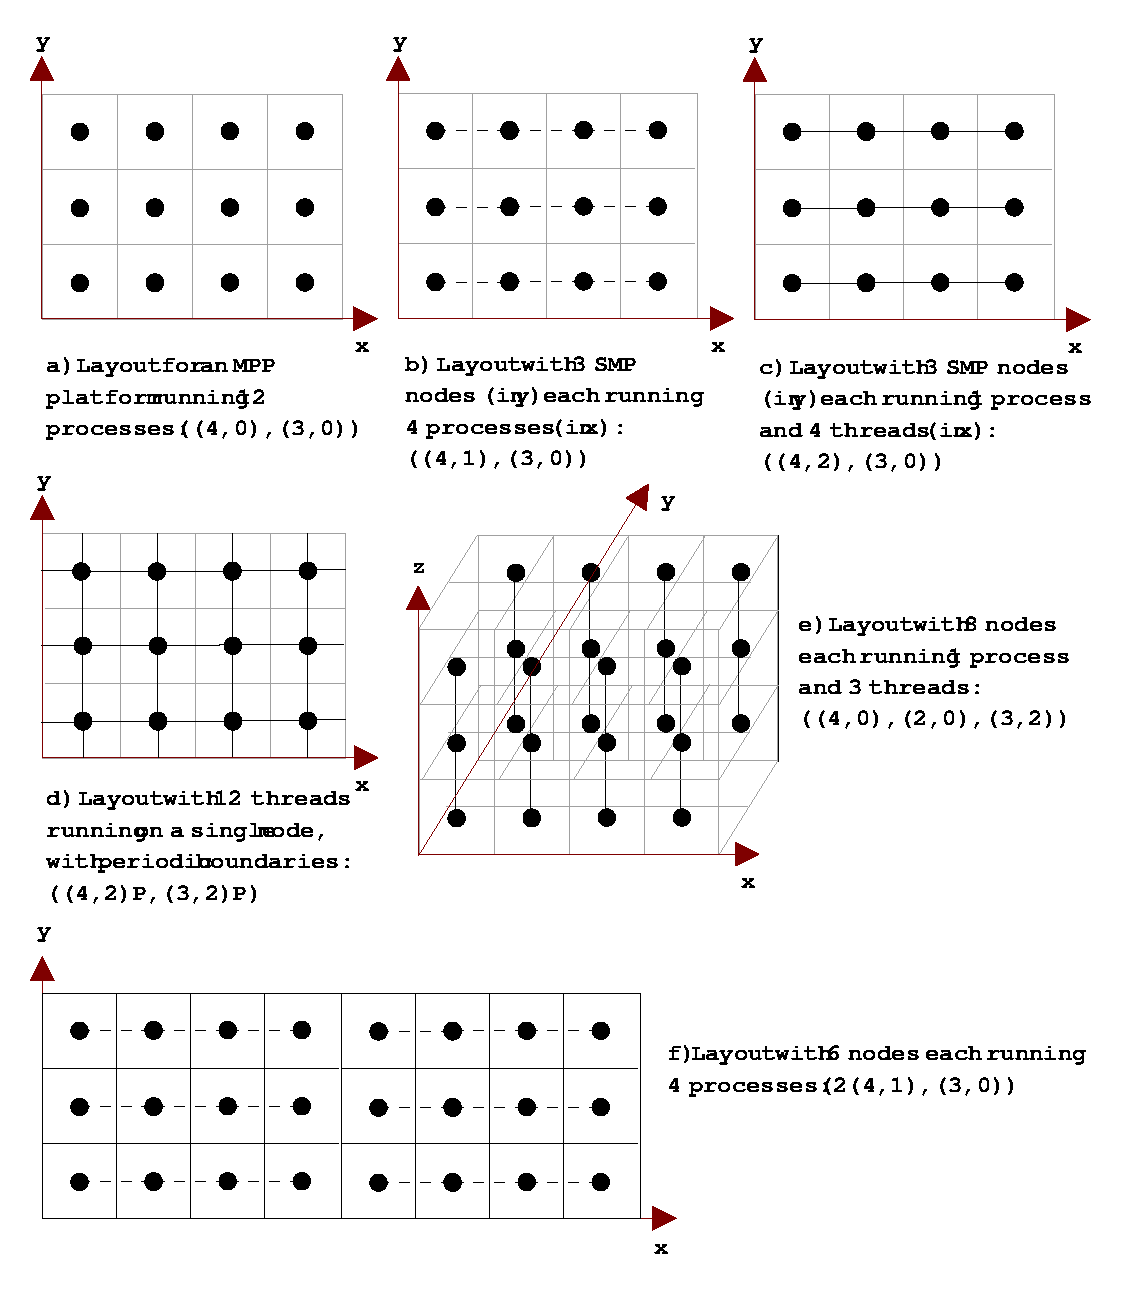
\includegraphics{Layout.eps}}
\end{figure}

Figure \ref{fig:layouts} shows number of examples of Layout objects.

When a Grid object is defined on a Layout, we require that the dimensions 
of the grid align with the dimensions of a Layout.  The superimposition
of a Grid on a Layout is shown in Figure \ref~{fig:gridlayout}.

\begin{figure}
\label{fig:gridlayout}
\scalebox{0.7}{\includegraphics{GridLayout.eps}}
\end{figure}

The user can request system resources either through a simple processor
ID list, or by defining a Layout.

More information on the ESMF machine model and programming model
is available in Section~\ref{sec:machine} and in the {\it ESMF
Implementation Report}.






